\section{Error Analysis}

\subsection{Error Overview}

Table~\ref{tab:error_overview} summarises the total number of test errors (misclassifications) for each experiment.

\begin{table}[H]
    \centering
    \caption{Total test-set errors per experiment (out of 3,798 samples).}
    \label{tab:error_overview}
    \begin{tabularx}{\textwidth}{l r r}
        \toprule
        \textbf{Experiment} & \textbf{Errors} & \textbf{Error Rate (\%)} \\
        \midrule
        EXP-1 BiLSTM         & 1,019 & 26.83 \\
        EXP-2 Frozen head    & 2,319 & 61.06 \\
        EXP-3 Full fine-tune & 557   & 14.67 \\
        \bottomrule
    \end{tabularx}
\end{table}

\subsection{Error Taxonomy}

We classify errors into three categories based on the relationship between the true label and the predicted label:

\begin{itemize}
    \item \textbf{Intensity errors:} The prediction is on the correct side of the sentiment spectrum (positive vs.\ negative) but at the wrong intensity level. Example: true label = \textit{Extremely Negative}, predicted = \textit{Negative}.
    \item \textbf{Neutral-boundary errors:} The model confuses a sentiment-bearing class with \textit{Neutral}, or vice versa. These indicate that the model fails to detect the presence or absence of a sentiment signal.
    \item \textbf{Polarity flips:} The model predicts a class on the opposite side of the sentiment spectrum from the true label (e.g.\ true = \textit{Positive}, predicted = \textit{Negative}). These are the most severe errors.
\end{itemize}

\subsection{Confusion Matrix Analysis}

\begin{figure}[H]
    \centering
    \begin{minipage}{0.48\textwidth}
        \centering
        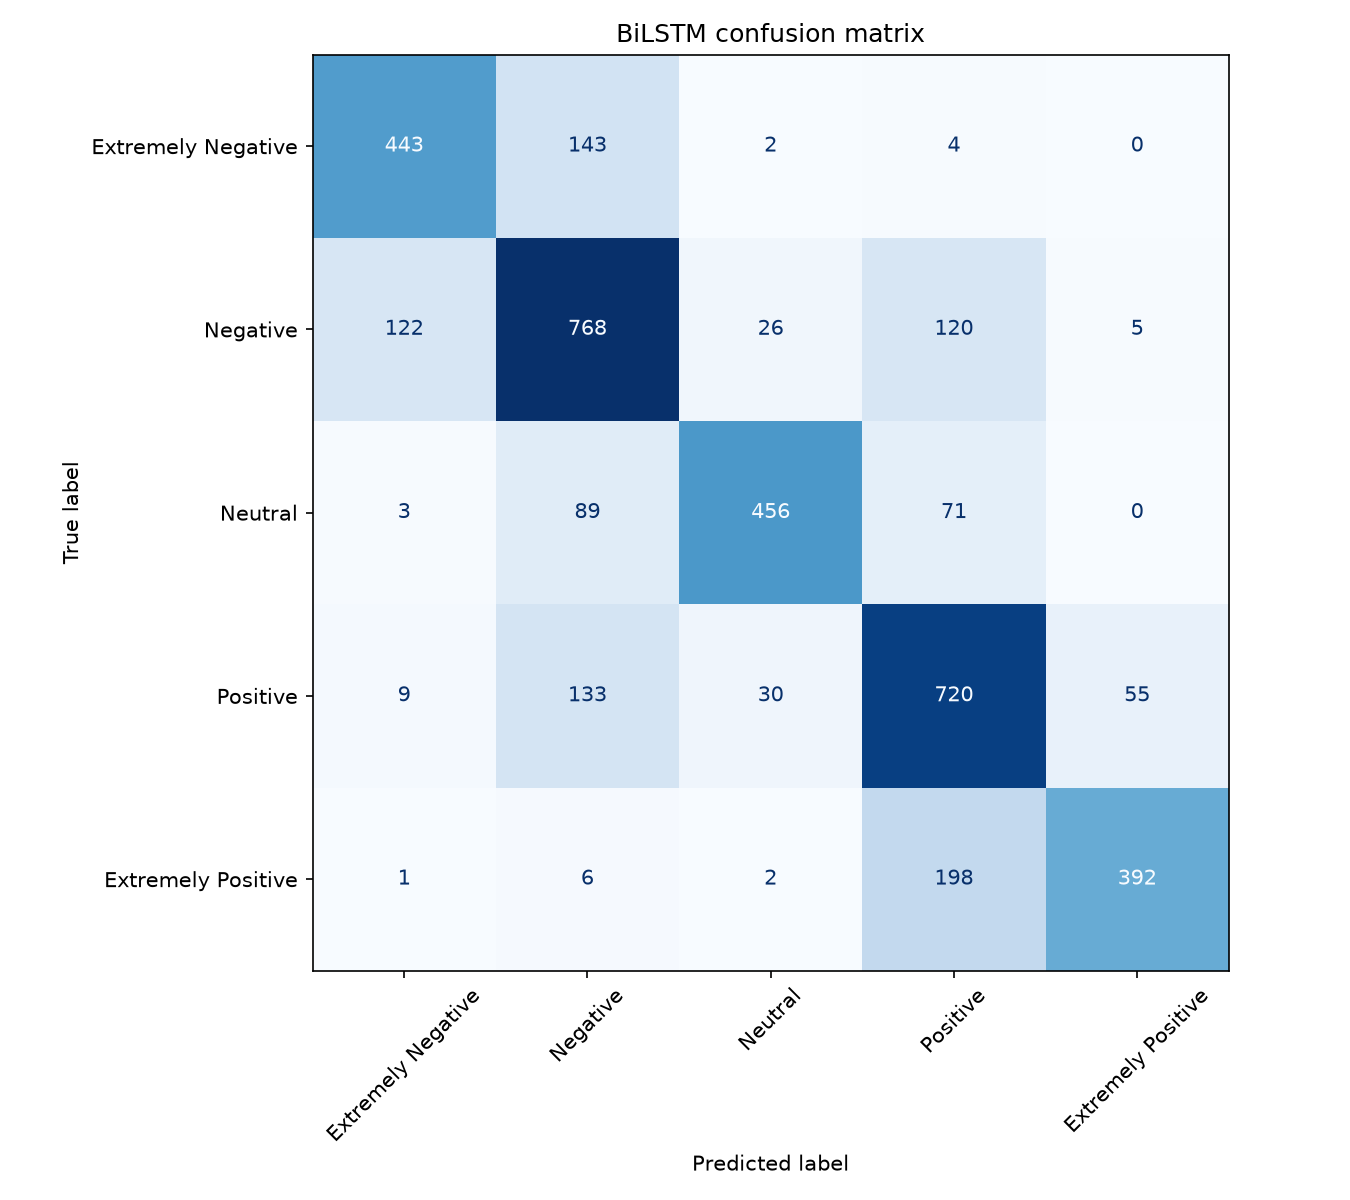
\includegraphics[width=\textwidth]{../../Assignment2/outputs/metrics/bilstm_confusion_matrix.png}
        \caption{Confusion matrix for EXP-1 (BiLSTM). Rows = true class, columns = predicted class.}
        \label{fig:cm_bilstm}
    \end{minipage}
    \hfill
    \begin{minipage}{0.48\textwidth}
        \centering
        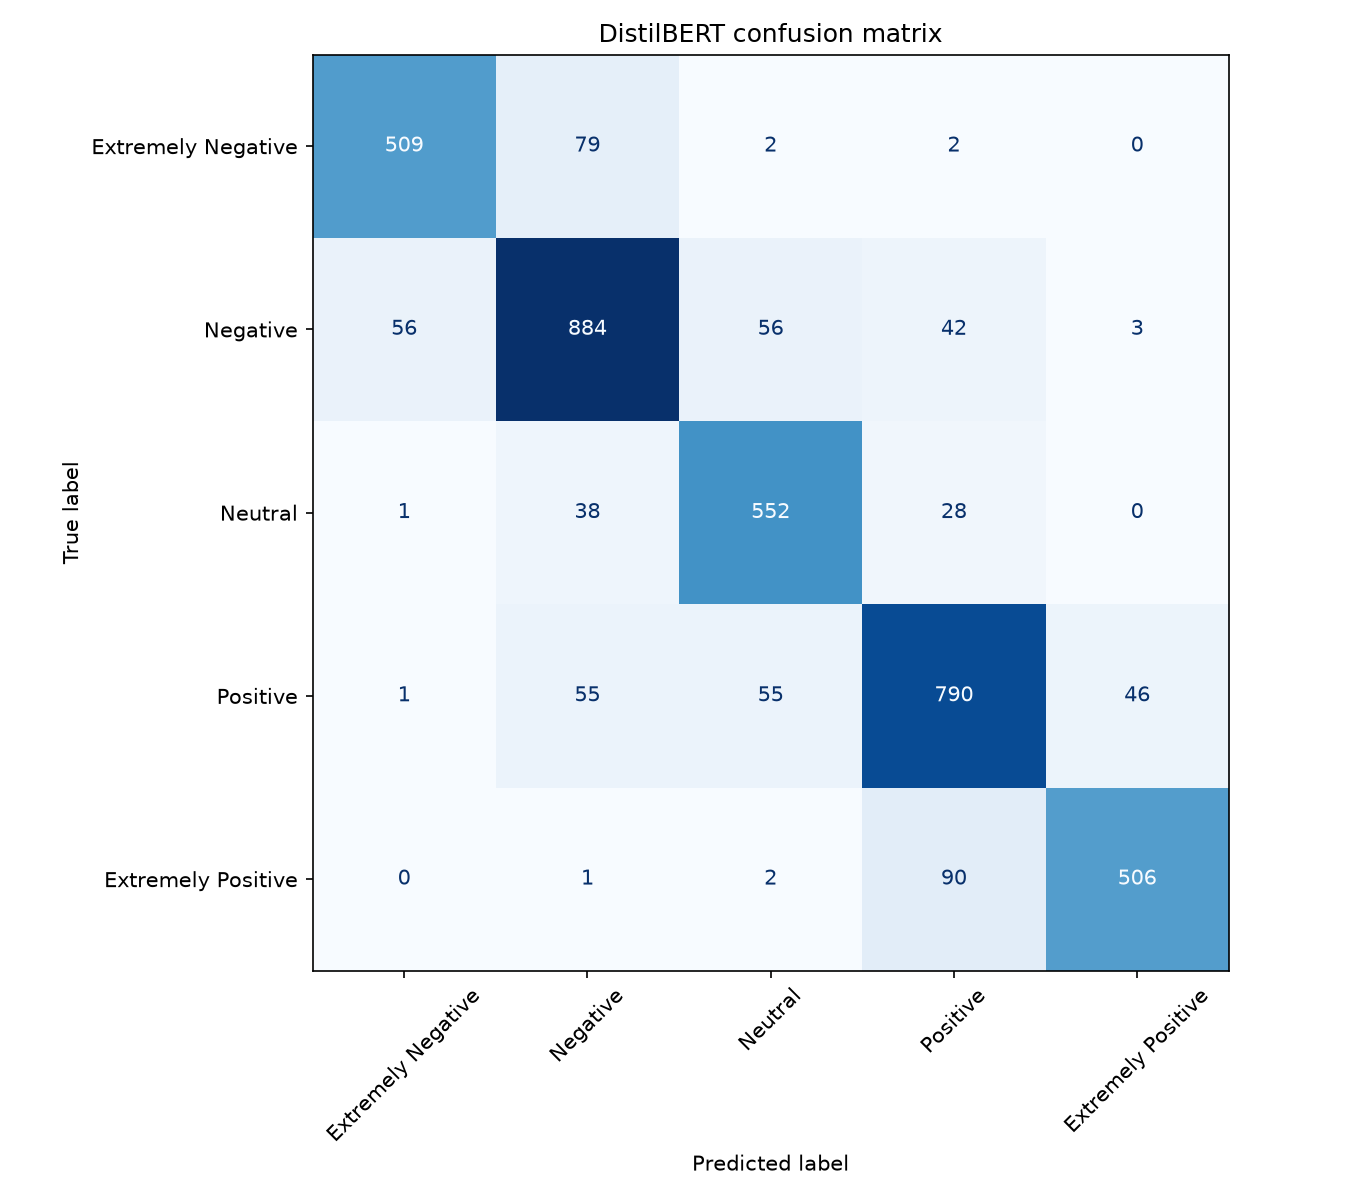
\includegraphics[width=\textwidth]{../../Assignment2/outputs/metrics/distilbert_confusion_matrix.png}
        \caption{Confusion matrix for EXP-3 (DistilBERT full). Rows = true class, columns = predicted class.}
        \label{fig:cm_distilbert}
    \end{minipage}
\end{figure}

\textbf{EXP-1 BiLSTM confusion patterns} (from the raw counts):
\begin{itemize}
    \item \textit{Negative} $\to$ \textit{Positive}: 120 cases (11.5\% of Negative samples). The model conflates \textit{Negative} with \textit{Positive}, suggesting that surface-level vocabulary cues occasionally dominate over sentiment direction.
    \item \textit{Positive} $\to$ \textit{Extremely Positive}: 55 cases; \textit{Extremely Positive} $\to$ \textit{Positive}: 198 cases. Classic intensity confusion in both directions.
    \item \textit{Neutral} $\to$ \textit{Negative}: 89 cases; informational/factual tweets pulled toward \textit{Negative} sentiment by pandemic-related vocabulary.
\end{itemize}

\textbf{EXP-3 DistilBERT full confusion patterns:}
\begin{itemize}
    \item The dominant off-diagonal entries are \textit{Extremely Negative}$\to$\textit{Negative} (79) and \textit{Negative}$\to$\textit{Neutral} (56) — a pattern of under-calling intensity.
    \item Polarity flips are rare: only 2 cases of \textit{Extremely Negative}$\to$\textit{Positive}/\textit{Extremely Positive} combined.
    \item The \textit{Extremely Positive}$\to$\textit{Positive} error (90 cases) is the largest off-diagonal entry, indicating intensity underestimation for the most positive class.
\end{itemize}

\subsection{Most Frequent Error Types by Class}

\begin{table}[H]
    \centering
    \caption{Most common misclassification for each true class in EXP-1 (BiLSTM) and EXP-3 (full fine-tune).}
    \label{tab:most_common_error}
    \begin{tabularx}{\textwidth}{l l l}
        \toprule
        \textbf{True Class} & \textbf{Most Common EXP-1 Error} & \textbf{Most Common EXP-3 Error} \\
        \midrule
        Ext.\ Negative   & $\to$ Negative (143)        & $\to$ Negative (79)  \\
        Negative          & $\to$ Positive (120)         & $\to$ Neutral (56)   \\
        Neutral           & $\to$ Negative (89)          & $\to$ Negative (38)  \\
        Positive          & $\to$ Negative (133)         & $\to$ Neutral (55)   \\
        Ext.\ Positive   & $\to$ Positive (198)         & $\to$ Positive (90)  \\
        \bottomrule
    \end{tabularx}
\end{table}

\subsection{Qualitative Failure Cases}

Table~\ref{tab:failure_cases} presents six representative test tweets where models made errors, illustrating the main failure modes.

\begin{table}[H]
    \centering
    \caption{Selected error cases with true label, model predictions, error category, and analysis.}
    \label{tab:failure_cases}
    \begin{tabularx}{\textwidth}{X l l l X}
        \toprule
        \textbf{Tweet (excerpt)} & \textbf{True} & \textbf{EXP-1} & \textbf{EXP-3} & \textbf{Analysis} \\
        \midrule
        ``The government has announced new measures but cases are still rising.''
            & Neg & Neu & Neu & Neutral-boundary: factual framing obscures negative sentiment \\
        \addlinespace
        ``INCREDIBLE news! First successful vaccine trial results!!!''
            & Ext.Pos & Pos & Ext.Pos & Intensity error (EXP-1): insufficient exclamation detection \\
        \addlinespace
        ``I'm so scared for my parents. This is a nightmare.''
            & Ext.Neg & Neg & Neg & Intensity underestimation; fear language not classified as extreme \\
        \addlinespace
        ``Supermarkets are running out of essentials. \#panic \#COVID19''
            & Neg & Pos & Neg & Polarity flip (EXP-1): `supermarket' and `essentials' may have positive training co-occurrences \\
        \addlinespace
        ``Schools closed, businesses shuttered, lives on hold. \#lockdown''
            & Neg & Neg & Neg & Correctly classified by both; unambiguous lexical cues \\
        \addlinespace
        ``Some people are helping their neighbours, others are hoarding. Mixed feelings.''
            & Neu & Neg & Neu & Neutral-boundary (EXP-1): `hoarding' triggers negative prediction despite overall neutral framing \\
        \bottomrule
    \end{tabularx}
\end{table}

\subsection{Label Ambiguity}

A proportion of errors may be attributable to genuine label ambiguity: tweets that could plausibly be annotated as either of two adjacent classes by different human annotators. The fine-grained 5-class scale exacerbates this, as intensity distinctions (e.g.\ \textit{Negative} vs.\ \textit{Extremely Negative}) are inherently subjective. These cases cannot be resolved by model improvement alone and represent an irreducible noise floor for this dataset.
